\documentclass[conference]{IEEEtran}
\IEEEoverridecommandlockouts
% The preceding line is only needed to identify funding in the first footnote. If that is unneeded, please comment it out.
\usepackage{cite}
\usepackage{amsmath,amssymb,amsfonts}
\usepackage{algorithmic}
\usepackage{graphicx}
\usepackage{textcomp}
\usepackage{xcolor}
\usepackage{tikz}
\usepackage{listings}
\usepackage{float}
\definecolor{lightgray}{rgb}{.95,.95,.95}
\definecolor{darkgray}{rgb}{.4,.4,.4}
\definecolor{purple}{rgb}{0.65, 0.12, 0.82}

% Tickz
\tikzstyle{startstop} = [rectangle, rounded corners, minimum width=3cm,
minimum height=1cm,text centered, draw=black, fill=red!30, text width = 5cm]
\tikzstyle{io} = [trapezium, trapezium left angle=70, trapezium right angle=110, minimum width=3cm, minimum height=1cm, text centered, draw=black, fill=blue!30]
\tikzstyle{process} = [rectangle, minimum width=3cm, minimum height=1cm, text centered, draw=black, fill=orange!30, text width = 5cm]
\tikzstyle{decision} = [diamond, minimum width=3cm, minimum height=1cm, text centered, draw=black, fill=green!30]
\tikzstyle{arrow} = [thick,->,>=stealth]



\lstdefinelanguage{JavaScript}{
  keywords={typeof, new, true, false, catch, function, return, null, catch, switch, var, let, const, if, in, while, do, else, case, break},
  keywordstyle=\color{blue}\bfseries,
  ndkeywords={class, export, boolean, throw, implements, import, this},
  ndkeywordstyle=\color{darkgray}\bfseries,
  identifierstyle=\color{black},
  sensitive=false,
  comment=[l]{//},
  morecomment=[s]{/*}{*/},
  commentstyle=\color{purple}\ttfamily,
  stringstyle=\color{red}\ttfamily,
  morestring=[b]',
  morestring=[b]"
}

\lstset{
   language=JavaScript,
   frame=single,
   backgroundcolor=\color{white},
   extendedchars=true,
   basicstyle=\scriptsize\ttfamily,
   showstringspaces=false,
   showspaces=false,
   numberstyle=\scriptsize,
   numbersep=9pt,
   tabsize=2,
   breaklines=true,
   showtabs=false,
   captionpos=b
}

\renewcommand{\lstlistingname}{Script.}

\def\BibTeX{{\rm B\kern-.05em{\sc i\kern-.025em b}\kern-.08em
    T\kern-.1667em\lower.7ex\hbox{E}\kern-.125emX}}
\begin{document}

\title{Analysis ChatGPT Potential: Transforming Software Development with AI Chat Bots\\
}

\makeatletter
\newcommand{\linebreakand}{%
  \end{@IEEEauthorhalign}
  \hfill\mbox{}\par
  \mbox{}\hfill\begin{@IEEEauthorhalign}
}



\author{
  \IEEEauthorblockN{Justine Winata Purwoko}
  \IEEEauthorblockA{\textit{Computer Science Department} \\
    \textit{School of Computer Science}\\
    \textit{Bina Nusantara University}\\
    Jakarta 11480, Indonesia\\
    justine.purwoko@binus.ac.id}
  \and
  \IEEEauthorblockN{Tegar Abdullah}
  \IEEEauthorblockA{\textit{Computer Science Department} \\
    \textit{School of Computer Science}\\
    \textit{Bina Nusantara University}\\
    Jakarta 11480, Indonesia\\
    tegar.abdullah@binus.ac.id}
  \and
   \IEEEauthorblockN{Budiman Wijaya}
  \IEEEauthorblockA{\textit{Computer Science Department} \\
    \textit{School of Computer Science}\\
    \textit{Bina Nusantara University}\\
    Jakarta 11480, Indonesia\\
    budiman.wijaya@binus.ac.id}
  \linebreakand 
  \IEEEauthorblockN{Alexander Agung Santoso Gunawan}
  \IEEEauthorblockA{\textit{Computer Science Department} \\
    \textit{School of Computer Science}\\
    \textit{Bina Nusantara University}\\
    Jakarta 11480, Indonesia\\
    agung@binus.edu}
  \and
  \IEEEauthorblockN{Karen Etania Saputra}
  \IEEEauthorblockA{\textit{Computer Science Department} \\
    \textit{School of Computer Science}\\
    \textit{Bina Nusantara University}\\
    Jakarta 11480, Indonesia\\
    karen.saputra@binus.edu}
}

\maketitle

\begin{abstract}
Artificial Intelligence (AI) is a technology that continues to develop and is increasingly being used in various aspects of life, including product and service development.  One type of AI that is developing rapidly is Chatbot, which is a computer program that can communicate with users via chat or voice applications.  However, there is still much debate among scientists and professionals about whether AI advancements like ChatGPT can help software engineer on working  daily task or even replace the work of software engineers.  So, on this occasion, we conduct research on whether AI (Artificial Intelligent) is capable of help software engineer and how far AI can assisting software engineer. In this study, we aim to evaluate the effectiveness of ChatGPT as a AI tool for code retrieval and its potential to help or replace software engineer. Our research methodology involves ChatGPT to refactor provided code, and make a simple application from scratch. The results of this research is, AI Chatbot model like ChatGPT cannot replace software developers 100\%. But it can actively help software developers in building a software on their daily life, especially in machine learning, application creation, and code refactoring.
\end{abstract}

\begin{IEEEkeywords}
Artificial Intelligent, Software Development, Chat Bot
\end{IEEEkeywords}

\section{Introduction}
Software development is a difficult, that's need a high level of ability and knowledge. Yet, new potential to increase the effectiveness of software development have emerged as a result of recent developments in artificial intelligence. Use of ChatGPT, a sophisticated language model trained on the GPT-3.5 architecture, is one such development. With encouraging outcomes, ChatGPT has been used to produce code for a number of software applications [1]. In this essay, we will investigate the use of ChatGPT to generate code for software applications and assess the usability and quality of the produced code.

ChatGPT is a potent tool that can produce code and natural language writing. ChatGPT has been trained in a variety of programming languages and can learn from a great amount of data. ChatGPT can produce code that follows the syntax and structure of several programming languages as a result [1].

When creating code with ChatGPT, input text is given to the model, which subsequently creates code depending on the input [2]. Human software engineers can then polish and enhance the generated code. The speed and effectiveness of software development can both be increased by this technique.

ChatGPT-produced software's usefulness and quality. The findings have been positive, with the program doing well in several tasks, including natural language processing, image recognition, and game development [2].
However, some people said, the software produced by ChatGPT still has certain limitations. In rare circumstances, the software may not operate as planned because of mistakes in the created code. Also, code produced by ChatGPT could not be as effective as code authored by real software developers [2]. This experiments aims to provide an overview of AI's benefits and limitations in software development by examining current literature and suggesting topics for further investigation [3]–[6]. 

In software testing, AI-driven techniques have the potential to revolutionize quality assurance work, speed up time to market, and enable businesses to create more complex software [8]–[10]. AI has been employed in various software development sectors, including project management, design, testing, and requirements engineering, with the potential to enhance software quality by automating repetitive tasks, identifying mistakes, and supporting decision-making [11].

AI's impact extends beyond traditional software development to industries such as e-commerce and IT Telecom, where AI-powered chatbots have been shown to improve customer satisfaction and service efficiency [12]–[15]. In web-based software development, AI and Machine Learning can lead to higher quality and efficiency in applications [16], [17]. Despite the advantages, developing AI-based chatbots can be challenging, with IBM Watson being identified as the best method among widely used Natural Language Understanding (NLU) techniques [18].

AI has also been employed in software development effort estimation, with the FNN approach demonstrating higher accuracy in overcoming uncertainty and vagueness [19]. Furthermore, natural language processing (NLP) advancements, such as GPT-3, GPT-4, and ChatGPT, have generated interest in their potential application in computer programming [20], [21]. ChatGPT has demonstrated promising results in producing code snippets [2], [22], [23]. ChatGPT can also help programmers with fixing their bug efficiently [1]. However, concerns have been raised about the quality and security of generated code [9], [25], [26].

AI offers numerous advantages in software development, but it is essential to consider the drawbacks, limitations, ethical, and transparency issues surrounding this technology. Therefore, in this research we have experiments that determine, can Chat GPT help or do programmer jobs in term of Software Engineering. This paper is arranged as follows: first, in section 2 we discuss the methodology of our experiments, such as how we conduct our experiments, prompting, or how we determine the results of our test. In section 3 we conducted the experiment that discussed in the methodology section. Finally in section 4, we  concluded  our  work with the experiment results and make an future improvement for the next research.  

\section{Methodology}
Through a series of tests, we ask the ChatGPT model to carry out various coding and software development-related activities as part of the study. The ChatGPT is available on https://chat.openai.com/ and can be used and open by all registered account. Our model is using 3.5 ChatGPT version so you can used for testing the available code. We use a simple prompting techniques for refactor, bug code, and machine learning like "refactor the below code with ...", etc. 

You can get all the source code and implementation information in our GitHub repository https://github.com/TinTinWinata/chat-gpt-analysis. The repository includes all of the tested's experiment, including refactor code, machine learning, simple application, and as well as the entire codebase, including the HTML, and JavaScript files.



\subsection{Refactor Code}
Our team provide a piece of smelly code with C\# language, that consist of Self Encapsulation Field and Inline Temp. You can see the explanation of smell code at refactoring guru (https://refactoring.guru/) and the code is available on our github repository. The piece of smell code that must be refactored sent to the ChatGPT model by using a simple prompt techniques. The code need to be refactored, and the ChatGPT model requested to submit a new and improved version of the code. The result of the refactored code getting analyzed with various scores like effectiveness and the correctness of code. 


\subsection{Simple Application}
The ChatGPT model asked to design a tic tac toe game in order to build a simple application. The ChatGPT model required to provide the JavaScript programming language code required to develop the application and ensure its proper operation. Furthermore, we challenged ChatGPT to add bots that can fight humans, as well as to make the bot smart enough to beat humans. The generated code then be tested by playing the game and determining who wins.

\vspace{0pt}
\begin{lstlisting}[caption={Simple Application Prompt}, basicstyle=\ttfamily,language=TeX]
can you make a tic tac toe game in javascript that comes with human vs bot game, where the human cannot win against the bot
\end{lstlisting}

From figure above, The prompt is a clear and concise question asking for the creation of a specific application—a tic-tac-toe game in JavaScript. The prompt further specifies that the game should include a human vs bot mode, where the human player cannot win against the bot player.

\subsection{Machine Learning}
The results of this machine learning testing is to create a machine learning code to predict whether the user has diabetes or not. This machine learning code prediction provided by naïve bayes approach to make the 2 type of classifications that is diabetes classification and not diabetes classification. 

\begin{figure}[H]
    \centering
    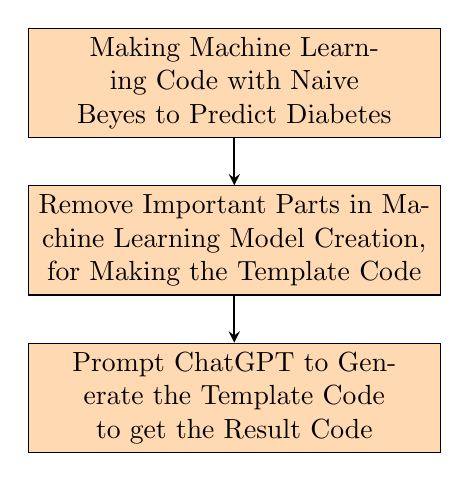
\begin{tikzpicture}[node distance=2cm]
        % \node (start) [startstop] {Start};
        \node (pro1) [process] {Making Machine Learning Code with Naive Beyes to Predict Diabetes};
        \node (pro2) [process, below of=pro1] {Remove Important Parts in Machine Learning Model Creation, for Making the Template Code };
        \node (pro3) [process, below of=pro2] {Prompt ChatGPT to Generate the Template Code to get the Result Code};
        % \node (stop) [startstop, below of=pro3] {Stop};
        % \draw [arrow] (start) -- (pro1);
        \draw [arrow] (pro1) -- (pro2);
        \draw [arrow] (pro2) -- (pro3);
        % \draw [arrow] (pro3) -- (stop);
    \end{tikzpicture}
    \caption{Flowchart of the Machine Learning Methodology Process}
\end{figure}

First, we create a machine learning code to predict whether user is diabetes or not. We're use naive bayes approach to make the code, the dataset that we used is diabetes data that you can found in kaggle and our github repository. This code provided with python language. We also use an advanced library like sklearn, numpy, matplotlib, and pandas so that we can see the performance of the ChatGPT whether it can use the library that has been provided or not. 

After we create the machine learning code, We discard the machine learning important modelling code and leave the rest of the code to the ChatGPT. When we discard important code we give a sign to ChatGPT to recreate the code at specific section. For making a fair comparison, we didn't remove the load dataset code because ChatGPT model didn't know and didn't see  the column and the value of dataset. 

\lstinputlisting[language=Python, caption={Template Code to be Filled by ChatGPT Model},showspaces=false, showstringspaces=false]{Machine Learning/template.py}

The ChatGPT model  built the machine learning model and generate the forecast of diabetes. The goal of this methodology is to make a comparison result of our first code who made by our team and the result of generated code by ChatGPT. Then, we analyzed the result of the prediction for the correct percentage using confussion matrix and compared the value result with the our team code.

\begin{lstlisting}[caption={Given Input \& Our Diabetes Result}, basicstyle=\scriptsize\ttfamily]
gender = 1
age = 19
hypertension = 0
heart_disease = 0
smoking_history = 0
bmi = 24.2
HbA1c_level = 5
blood_glucose_level = 130

You are not diabetes!
Accuracy score: 0.90488
\end{lstlisting}

\section{Experiments \& Results}
We outline the experiments conducted to address our research questions in this experiments and result   section. In Section A, we look at how ChatGPT may assist programmers with code refactoring. We examine ChatGPT's capabilities for basic application generation and machine learning prediction in Sections B and C. Refactor Code.

\subsection{Refactor Code}
Leveraging the power of Artificial Intelligence, we conducted experiments using C\#. Based on the experiment results, ChatGPT provides best practices for code refactoring, including separating logic into multiple functions, avoiding code duplication, and more.

\lstinputlisting[language={[Sharp]C}, caption={Unfactored Code}]{Refactor/before.cs}

\lstinputlisting[language={[Sharp]C}, caption={Refactored Code}]{Refactor/after.cs}

The figure above shows ChatGPT improved the structure, readability, and adherence to best practices in application development. As we can see as a languange modelling, ChatGPT can know where's the smell code and implemented a refactored code. They remove the Self Encapsulation Field smell code and implement getter and setter in the code. But for the inline temp smell in the previous code, the ChatGPT is remove the code and changed to only deducted the current money. This getting be a problem, because initially we want to get our money but instead, the money is not received and produce a void return. 

The results generated by ChatGPT also align with universal principles and standards in application development. The resulting code is well-structured, easier to test, and maintainable. Overall, ChatGPT can greatly assist in the software development process by addressing smell code and enhancing the overall code quality of applications. However, the code created by ChatGPT may contain mistakes and misconceptions. As developers, it is critical that we comprehend and properly evaluate the code generated by ChatGPT.



\subsection{Simple Application}
The analysis focuses on how well ChatGPT generates code that can execute properly and adhere to standards. We put it to the test by giving ChatGPT a prompt to create a game of tic-tac-toe that uses HTML, CSS, and JavaScript programming languages. As a result, when we play the game of tic-tac-toe, the ChatGPT model is able to accomplish this and pass the test.

We also resent the prompt to ChatGPT to enable human vs. bot play in the game. We also asked it to make the bot as intelligent as possible so that it could outplay people at the game of tic-tac-toe. It turns out ChatGPT uses the mini-max algorithm to decide the best moves in order to guarantee that the bot always wins or at least manages to achieve a draw when playing the tic-tac-toe game.

This experiment demonstrated ChatGPT's flexibility in implementing complex algorithms in addition to producing functional code. ChatGPT successfully developed a fully playable tic-tac-toe game with a clever bot opponent by combining its knowledge of game theory and programming languages. This highlights the model's potential even more as a useful tool for creating interactive programs and games.

\lstinputlisting[language={JavaScript}, caption={Mini-Max Algorithm Made by ChatGPT}, firstline=104, lastline=132]{Simple Application/tic-tac-toe.js}


\vspace{-5pt}

\begin{figure}[H]
\centerline{\includegraphics[width=0.3\linewidth]{Simple Application/draw.png}}
\caption{Bot draw against human.}
\label{simple app draw}
\end{figure}

\vspace{-10pt}

\begin{figure}[H]
\centerline{\includegraphics[width=0.3\linewidth]{Simple Application/won.png}}
\caption{Bot won against human.}
\label{simple app won}
\end{figure}

\subsection{Machine Learning}
Our machine learning research centered on using ChatGPT to generate code that could determine whether user input suggests diabetes. According to the methodology section, we used machine learning code templates that were already created to be filled in by ChatGPT model.

\lstinputlisting[language=Python, caption={Model Code that Filled from Template by ChatGPT},showspaces=false, showstringspaces=false]{Machine Learning/chat-gpt-model-only.py}

\begin{lstlisting}[caption={Given Input \& ChatGPT Diabetes Result}, basicstyle=\scriptsize\ttfamily]
gender = 1
age = 19
hypertension = 0
heart_disease = 0
smoking_history = 0
bmi = 24.2
HbA1c_level = 5
blood_glucose_level = 130

You are not diabetes!
Accuracy score: 0.90488
\end{lstlisting}

Based on the user's input, this code was used to determine how likely it was that they would get diabetes. We conclude the code that is generated by ChatGPT has the same answer as the human code made. The code also has 90.49\% accuracy percentage to predict whether user is diabetes or not, the same percentage number that the human-created code also have.

\begin{figure}[htbp]
\centerline{\includegraphics[width=1\linewidth]{Machine Learning/Diabetes.png}}
\caption{}
\label{simple app won}
\end{figure}

Figure above, shows the confusion matrix for both human-coded and ChatGPT-generated solutions to give the visualisation of performance. This visual depiction allows us to evaluate the true positives, true negatives, false positives, and false negatives. By comparing the confusion matrices, ChatGPT performs similarly to human code in terms of accuracy.

Overall, the machine learning tests showed how well ChatGPT generates code for machine learning tasks, particularly for determining whether or not a person has diabetes. These findings demonstrate ChatGPT's potential as a useful tool for tackling difficult machine learning challenges. ChatGPT's ability to create accurate code enables it to aid developers and academics in efficiently handling challenging machine learning problems.

\section{Conclusion}

The trials demonstrated ChatGPT's potential as a useful tool in software development. Developers may use its language generating features to help with bug patches, code restructuring, machine learning jobs, and the creation of small apps. While there are still limits and potential for improvement, ChatGPT provides intriguing opportunities to increase the efficacy and efficiency of software development processes.

While the experiments demonstrated ChatGPT's promise, it is crucial to recognize its limits. In rare circumstances, the produced code may contain flaws or fail to behave as planned, emphasizing the importance of human supervision and improvement. Furthermore, the model's reliance on training data raises worries about possible biases or weaknesses in the resulting code.

Despite their own limitations, it is impossible to ignore ChatGPT's potential influence on software development ethic. The model's capacity as a helpful tool for developers is demonstrated by its capacity to generate code that complies with industry standards and carry out challenging programming tasks. This will not replace 100\% software development but With further development and improvement, ChatGPT has the potential to enhance and streamline software development workflows, allowing developers to work more efficiently and creatively.

ChatGPT model already comes up with new version, namely version ChatGPT 4 and produces better result than ChatGPT 3.5. Because, there's are limitation in our research, all the research above is using ChatGPT 3.5 and we cannot see the different between those version. For the purpose of future research, we suggest to make a comparison between another model like ChatGPT 4 or Google Bard. So, future research not only finding the function of ChatGPT model on software development but we encourage to find the best model to suit up software engineer to do a daily programmer task by comparing all existing model.  

\begin{thebibliography}{00}
\bibitem{b1} N. M. S. Surameery and M. Y. Shakor, “Use Chat GPT to Solve Programming Bugs,” International Journal of Information technology and Computer Engineering, no. 31, pp. 17–22, Jan. 2023, doi: 10.55529/ijitc.31.17.22. 
\bibitem{b2} H. Tian et al., “Is ChatGPT the Ultimate Programming Assistant -- How far is it?,” Apr. 2023. 
\bibitem{b3} Senthil Velan S., Introducing Artificial Intelligence Agents to the Empirical Measurement of Design Properties for Aspect Oriented Software Development. IEEE, 2019. 
\bibitem{b4} R. Feldt, F. G. de Oliveira Neto, and R. Torkar, “Ways of applying artificial intelligence in software engineering,” Association for Computing Machinery (ACM), May 2018, pp. 35–41. doi: 10.1145/3194104.3194109. 
\bibitem{b5} P. Vrentuša, “USING ARTIFICIAL INTELLIGENCE IN SOFTWARE DEVELOPMENT: A CASE ANALYSIS,” 2023. 
\bibitem{b6} W. Haider, M. Jawad, Y. Hafeez, F. Burhan Ahmad, S. Ali, and M. Numan Rafi, “Improving Requirement Prioritization and Traceability using Artificial Intelligence Technique for Global Software Development,” 2019. 
\bibitem{b7} E. Khanna, R. Popli, and N. Chauhan, “Artificial Intelligence based Risk Management Framework for Distributed Agile Software Development,” in 2021 8th International Conference on Signal Processing and Integrated Networks (SPIN), IEEE, Aug. 2021, pp. 657–660. doi: 10.1109/SPIN52536.2021.9566000. 
\bibitem{b8} D. G. Lee and Y. S. Seo, “Improving bug report triage performance using artificial intelligence based document generation model,” Human-centric Computing and Information Sciences, vol. 10, no. 1, Dec. 2020, doi: 10.1186/s13673-020-00229-7. 
\bibitem{b9} H. Hourani, A. Hammad, and M. Lafi, “The Impact of Artificial Intelligence on Software Testing,” in 2019 IEEE Jordan International Joint Conference on Electrical Engineering and Information Technology (JEEIT), IEEE, Apr. 2019, pp. 565–570. doi: 10.1109/JEEIT.2019.8717439. 
\bibitem{b10} Z. Khaliq, S. U. Farooq, and D. A. Khan, “Artificial Intelligence in Software Testing: Impact, Problems, Challenges and Prospect,” Jan. 2022, {Online}. Available: http://arxiv.org/abs/2201.05371 
\bibitem{b11} D. Kothari, “How Artificial Intelligence Accelerates Software Development,” in International Research Journal of Engineering and Technology (IRJET), 2019, pp. 1392–1394. 
\bibitem{b12} X. Song, S. Yang, Z. Huang, and T. Huang, “The Application of Artificial Intelligence in Electronic Commerce,” J Phys Conf Ser, vol. 1302, no. 3, p. 032030, Aug. 2019, doi: 10.1088/1742-6596/1302/3/032030. 
\bibitem{b13} M. M. Khan, “Development of An e-commerce Sales Chatbot,” in 2020 IEEE 17th International Conference on Smart Communities: Improving Quality of Life Using ICT, IoT and AI (HONET), IEEE, Dec. 2020, pp. 173–176. doi: 10.1109/HONET50430.2020.9322667. 
\bibitem{b14} M. Rakhra et al., “E-Commerce Assistance with a Smart Chatbot using Artificial Intelligence,” in 2021 2nd International Conference on Intelligent Engineering and Management (ICIEM), IEEE, Apr. 2021, pp. 144–148. doi: 10.1109/ICIEM51511.2021.9445316. 
\bibitem{b15} M. G. C. P, A. Srivastava, S. Chakraborty, A. Ghosh, and H. Raj, “Development of Information Technology Telecom Chatbot: An Artificial Intelligence and Machine Learning Approach,” in 2021 2nd International Conference on Intelligent Engineering and Management (ICIEM), IEEE, Apr. 2021, pp. 216–221. doi: 10.1109/ICIEM51511.2021.9445354. 
\bibitem{b16} K. Wakil and D. N. A. Jawawi, “Intelligent Web Applications as Future Generation of Web Applications,” Scientific Journal of Informatics, vol. 6, no. 2, pp. 2407–7658, 2019, {Online}. Available: http://journal.unnes.ac.id/nju/index.php/sji 
\bibitem{b17} V. Le et al., “A web-based AI assistant Application using Python and JavaScript,” Nonprofit Administration and Management Commons, Public Administration Commons, Public Health Commons, Social Media Commons, and the Sociology of Culture Commons. {Online}. Available: https://commons.clarku.edu/sps\_masters\_papers/63 
\bibitem{b18} A. Abdellatif, K. Badran, D. E. Costa, and E. Shihab, “A Comparison of Natural Language Understanding Platforms for Chatbots in Software Engineering,” IEEE Transactions on Software Engineering, vol. 48, no. 8, pp. 3087–3102, Aug. 2022, doi: 10.1109/TSE.2021.3078384. 
\bibitem{b19} A. B. Nassif, M. Azzeh, A. Idri, and A. Abran, “Software Development Effort Estimation Using Regression Fuzzy Models,” Comput Intell Neurosci, vol. 2019, pp. 1–17, Feb. 2019, doi: 10.1155/2019/8367214. 
\bibitem{b20} A. Zarifhonarvar, “Economics of ChatGPT: A Labor Market View on the Occupational Impact of Artificial Intelligence.” {Online}. Available: https://ssrn.com/abstract=4350925 
\bibitem{b21} S. Biswas, “Role of ChatGPT in Computer Programming,” Mesopotamian Journal of Computer Science, pp. 8–16, Jan. 2023, doi: 10.58496/MJCSC/2023/002. 
\bibitem{b22} A. Kashefi and T. Mukerji, “ChatGPT for Programming Numerical Methods,” Mar. 2023. 
\bibitem{b23} N. Perry, M. Srivastava, D. Kumar, and D. Boneh, “Do Users Write More Insecure Code with AI Assistants?,” Nov. 2022. 
\bibitem{b24} S. Bordt and U. von Luxburg, “ChatGPT Participates in a Computer Science Exam,” Mar. 2023. 
\bibitem{b25} Dhaya Sindhu Battina, “Artificial Intelligence in Software Test Automation: A Systematic Literature Review,” 2019. {Online}. Available: www.jetir.org 
\bibitem{b26} R. Khoury, A. R. Avila, J. Brunelle, and B. M. Camara, “How Secure is Code Generated by ChatGPT?,” Apr. 2023. 
\bibitem{b27} V. Vakkuri, K. K. Kemell, J. Tolvanen, M. Jantunen, E. Halme, and P. Abrahamsson, “How Do Software Companies Deal with Artificial Intelligence Ethics? A Gap Analysis,” in ACM International Conference Proceeding Series, Association for Computing Machinery, Jun. 2022, pp. 100–109. doi: 10.1145/3530019.3530030.
\end{thebibliography}

\end{document}

